% Options for packages loaded elsewhere
\PassOptionsToPackage{unicode}{hyperref}
\PassOptionsToPackage{hyphens}{url}
%
\documentclass[
]{article}
\usepackage{lmodern}
\usepackage{amssymb,amsmath}
\usepackage{ifxetex,ifluatex}
\ifnum 0\ifxetex 1\fi\ifluatex 1\fi=0 % if pdftex
  \usepackage[T1]{fontenc}
  \usepackage[utf8]{inputenc}
  \usepackage{textcomp} % provide euro and other symbols
\else % if luatex or xetex
  \usepackage{unicode-math}
  \defaultfontfeatures{Scale=MatchLowercase}
  \defaultfontfeatures[\rmfamily]{Ligatures=TeX,Scale=1}
\fi
% Use upquote if available, for straight quotes in verbatim environments
\IfFileExists{upquote.sty}{\usepackage{upquote}}{}
\IfFileExists{microtype.sty}{% use microtype if available
  \usepackage[]{microtype}
  \UseMicrotypeSet[protrusion]{basicmath} % disable protrusion for tt fonts
}{}
\makeatletter
\@ifundefined{KOMAClassName}{% if non-KOMA class
  \IfFileExists{parskip.sty}{%
    \usepackage{parskip}
  }{% else
    \setlength{\parindent}{0pt}
    \setlength{\parskip}{6pt plus 2pt minus 1pt}}
}{% if KOMA class
  \KOMAoptions{parskip=half}}
\makeatother
\usepackage{xcolor}
\IfFileExists{xurl.sty}{\usepackage{xurl}}{} % add URL line breaks if available
\IfFileExists{bookmark.sty}{\usepackage{bookmark}}{\usepackage{hyperref}}
\hypersetup{
  hidelinks,
  pdfcreator={LaTeX via pandoc}}
\urlstyle{same} % disable monospaced font for URLs
\usepackage[margin=1in]{geometry}
\usepackage{longtable,booktabs}
% Correct order of tables after \paragraph or \subparagraph
\usepackage{etoolbox}
\makeatletter
\patchcmd\longtable{\par}{\if@noskipsec\mbox{}\fi\par}{}{}
\makeatother
% Allow footnotes in longtable head/foot
\IfFileExists{footnotehyper.sty}{\usepackage{footnotehyper}}{\usepackage{footnote}}
\makesavenoteenv{longtable}
\usepackage{graphicx,grffile}
\makeatletter
\def\maxwidth{\ifdim\Gin@nat@width>\linewidth\linewidth\else\Gin@nat@width\fi}
\def\maxheight{\ifdim\Gin@nat@height>\textheight\textheight\else\Gin@nat@height\fi}
\makeatother
% Scale images if necessary, so that they will not overflow the page
% margins by default, and it is still possible to overwrite the defaults
% using explicit options in \includegraphics[width, height, ...]{}
\setkeys{Gin}{width=\maxwidth,height=\maxheight,keepaspectratio}
% Set default figure placement to htbp
\makeatletter
\def\fps@figure{htbp}
\makeatother
\setlength{\emergencystretch}{3em} % prevent overfull lines
\providecommand{\tightlist}{%
  \setlength{\itemsep}{0pt}\setlength{\parskip}{0pt}}
\setcounter{secnumdepth}{-\maxdimen} % remove section numbering

\author{}
\date{\vspace{-2.5em}}

\begin{document}

\hypertarget{technical-assessment-document}{%
\section{Technical Assessment
Document}\label{technical-assessment-document}}

The given data represents financial information about insurance firms,
and is multivariate in nature. Firm size, changing business profiles,
and outliers are important in the analysis of this data. Using the
programming language R, I have provided an exploratory analysis. The
source code can be found in the \texttt{./src/analysis.R} file in this
repository.

\hypertarget{analyses}{%
\subsection{Analyses}\label{analyses}}

As the data is presented in a time series format, this is useful to pick
out trends over time.

\hypertarget{gross-written-premium-gwp}{%
\subsubsection{Gross Written Premium
(GWP)}\label{gross-written-premium-gwp}}

Most of the firms in this data set have a GWP of around £920m, taking
the average of all values of GWP. To isolate the largest firms, I chose
to filter the firms to display by those firms which have on average more
than £1000m GWP over the four year period in question (2016-2020). We
can display temporal trends of these firms.

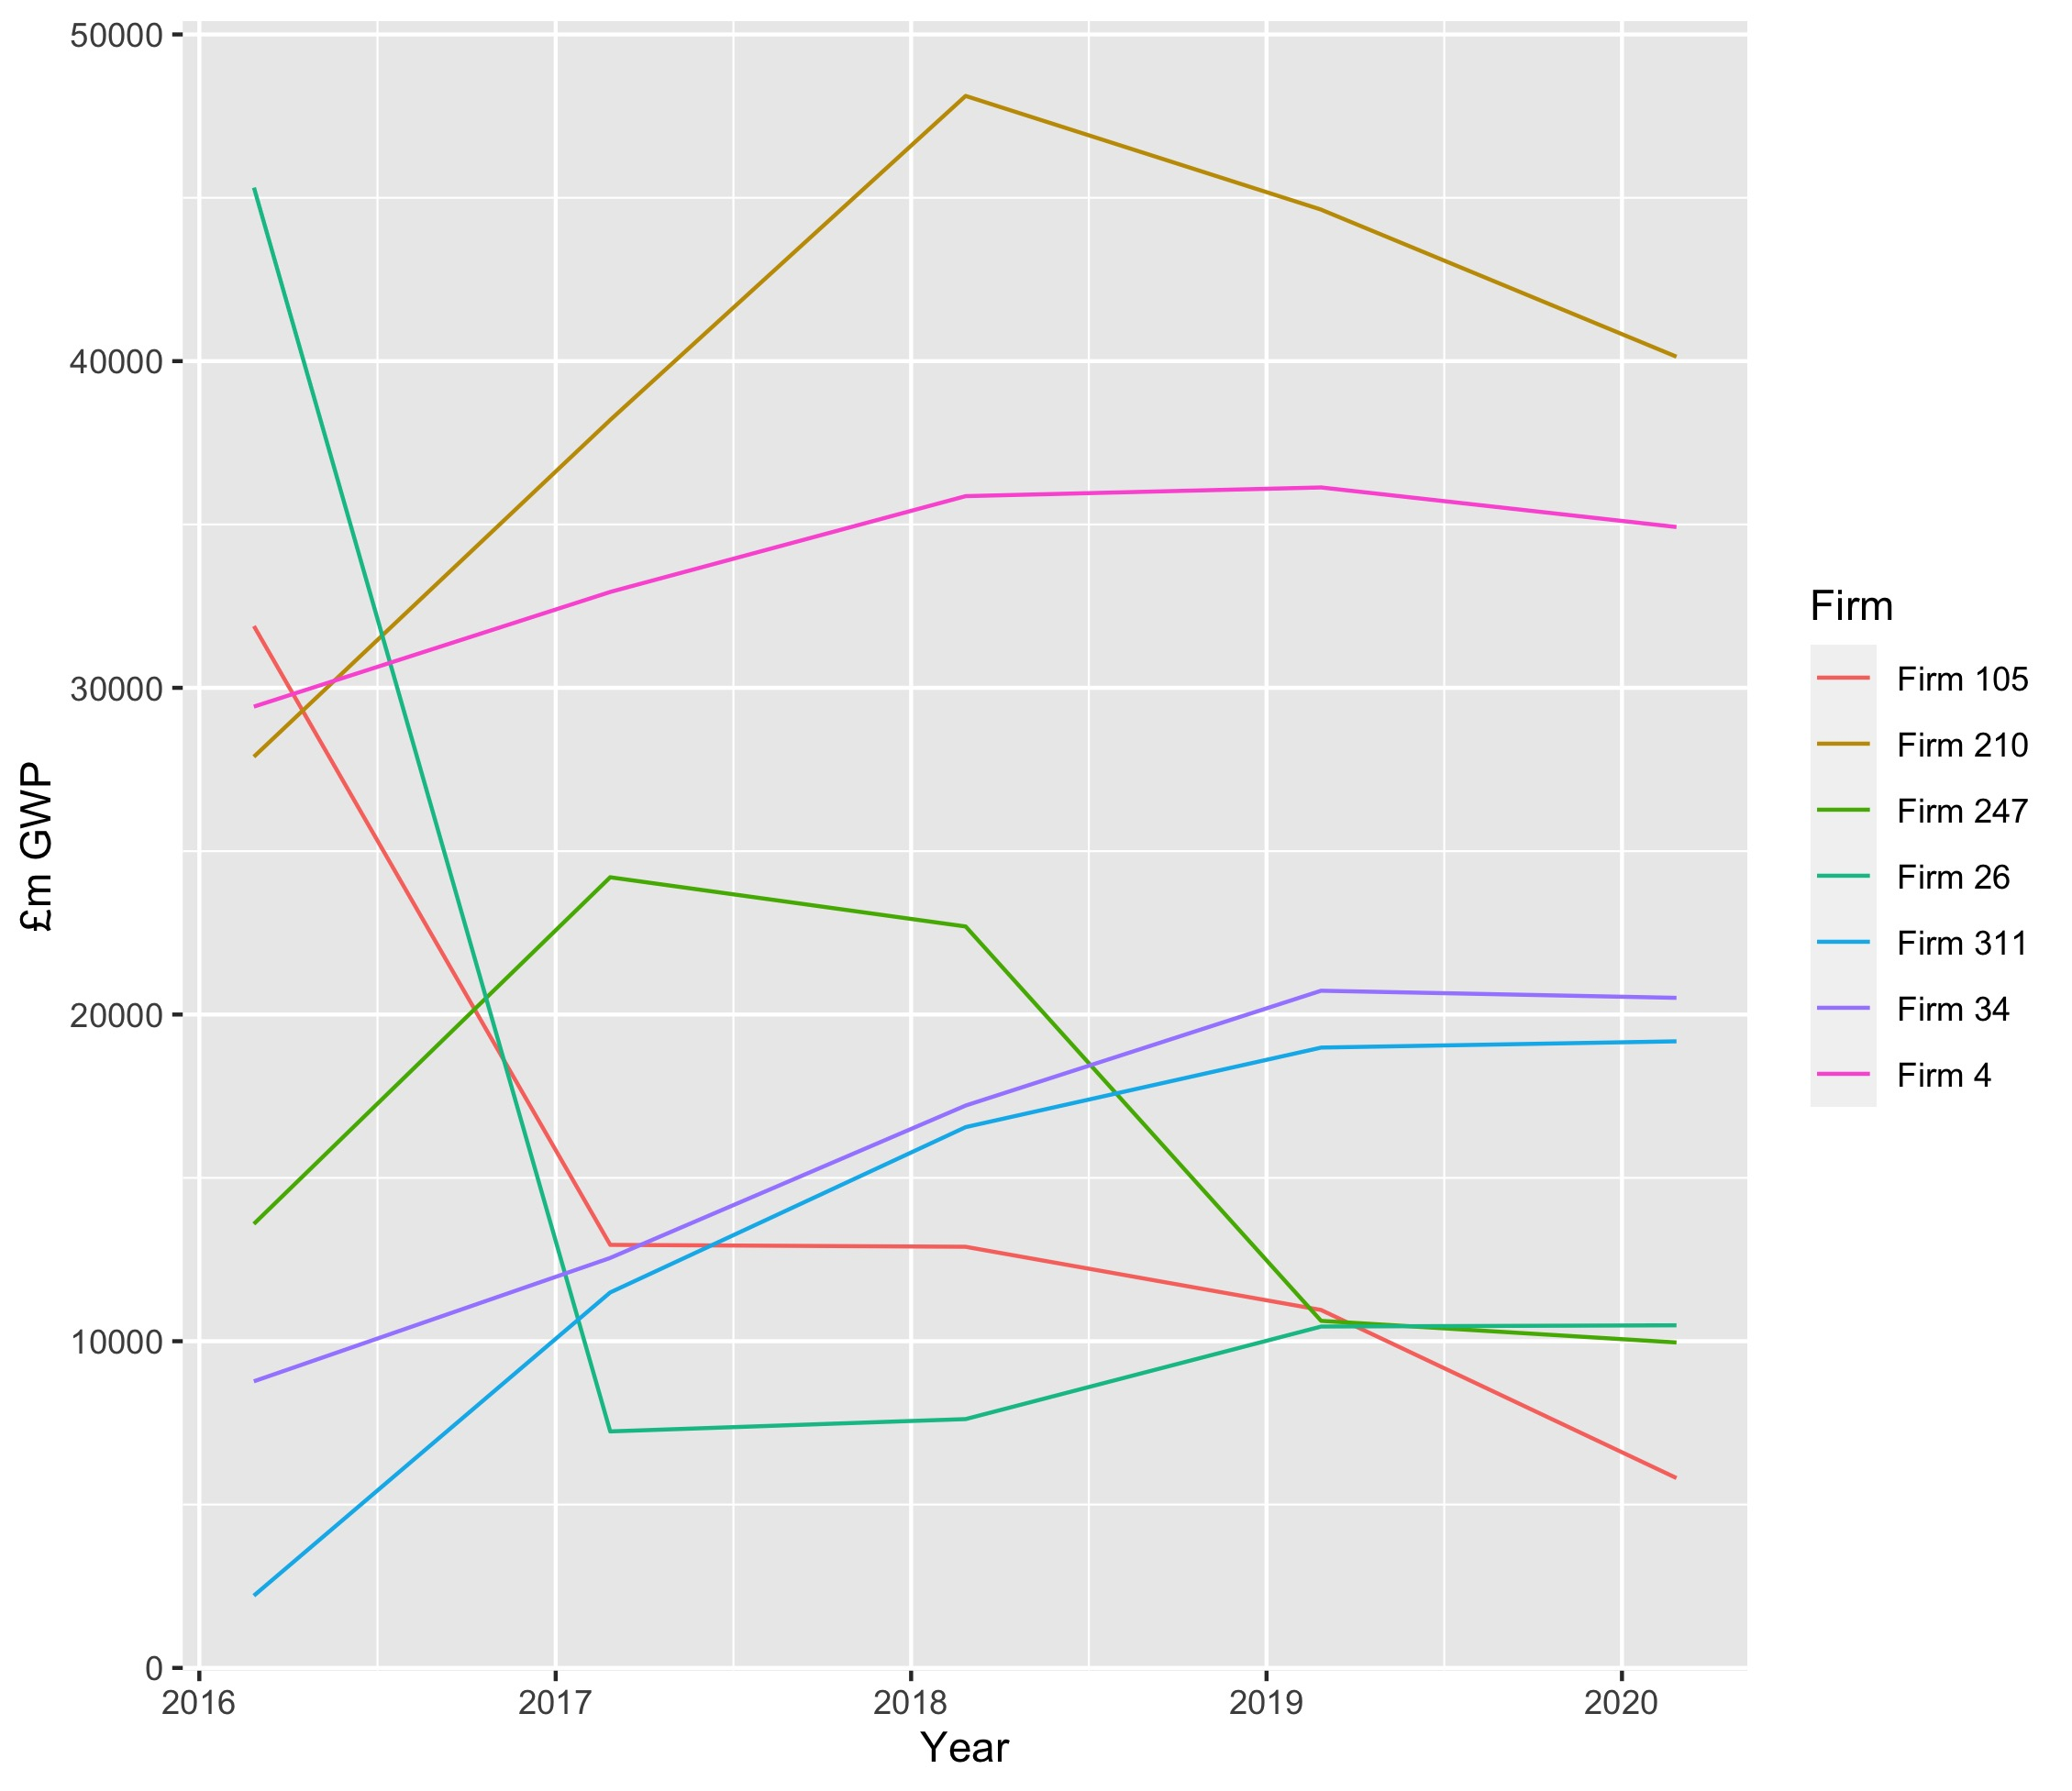
\includegraphics[width=1\linewidth]{../figs/gwp_plot_avg_10000}

The image is a little cluttered, and we can be guided in interpretation
of this figure by looking at the variance over time for each firm.

\begin{longtable}[]{@{}lr@{}}
\toprule
Firm & Variance in GWP over time\tabularnewline
\midrule
\endhead
Firm 26 & 266754424\tabularnewline
Firm 105 & 98647001\tabularnewline
Firm 210 & 59285334\tabularnewline
Firm 311 & 50751941\tabularnewline
Firm 247 & 45760946\tabularnewline
Firm 73 & 32923070\tabularnewline
\bottomrule
\end{longtable}

Each of the firms in this image would warrant further investigation, but
especially firm 26, which has an order of magnitude greater variance in
GWP than any other firm. This is shown by the large drop in GWP from
2016 to 2017.

\hypertarget{net-written-premium-nwp}{%
\subsubsection{Net Written Premium
(NWP)}\label{net-written-premium-nwp}}

NWP is significantly correlated with GWP (p \textless{} 0.05), and so as
expected the trajectories of each of the largest firms remain similar.
Below is a regression of NWP against GWP, showing their high
correlation. The red line is the x = y line; where a firm is not
reinsuring anything. Most firms are reinsuring something, hence why the
grey-dashed line (\textasciitilde{} 0.85 slope) is shallower than the
1:1 line. The firms that fall below this line are the most interesting
as they are reinsuring more than the average.

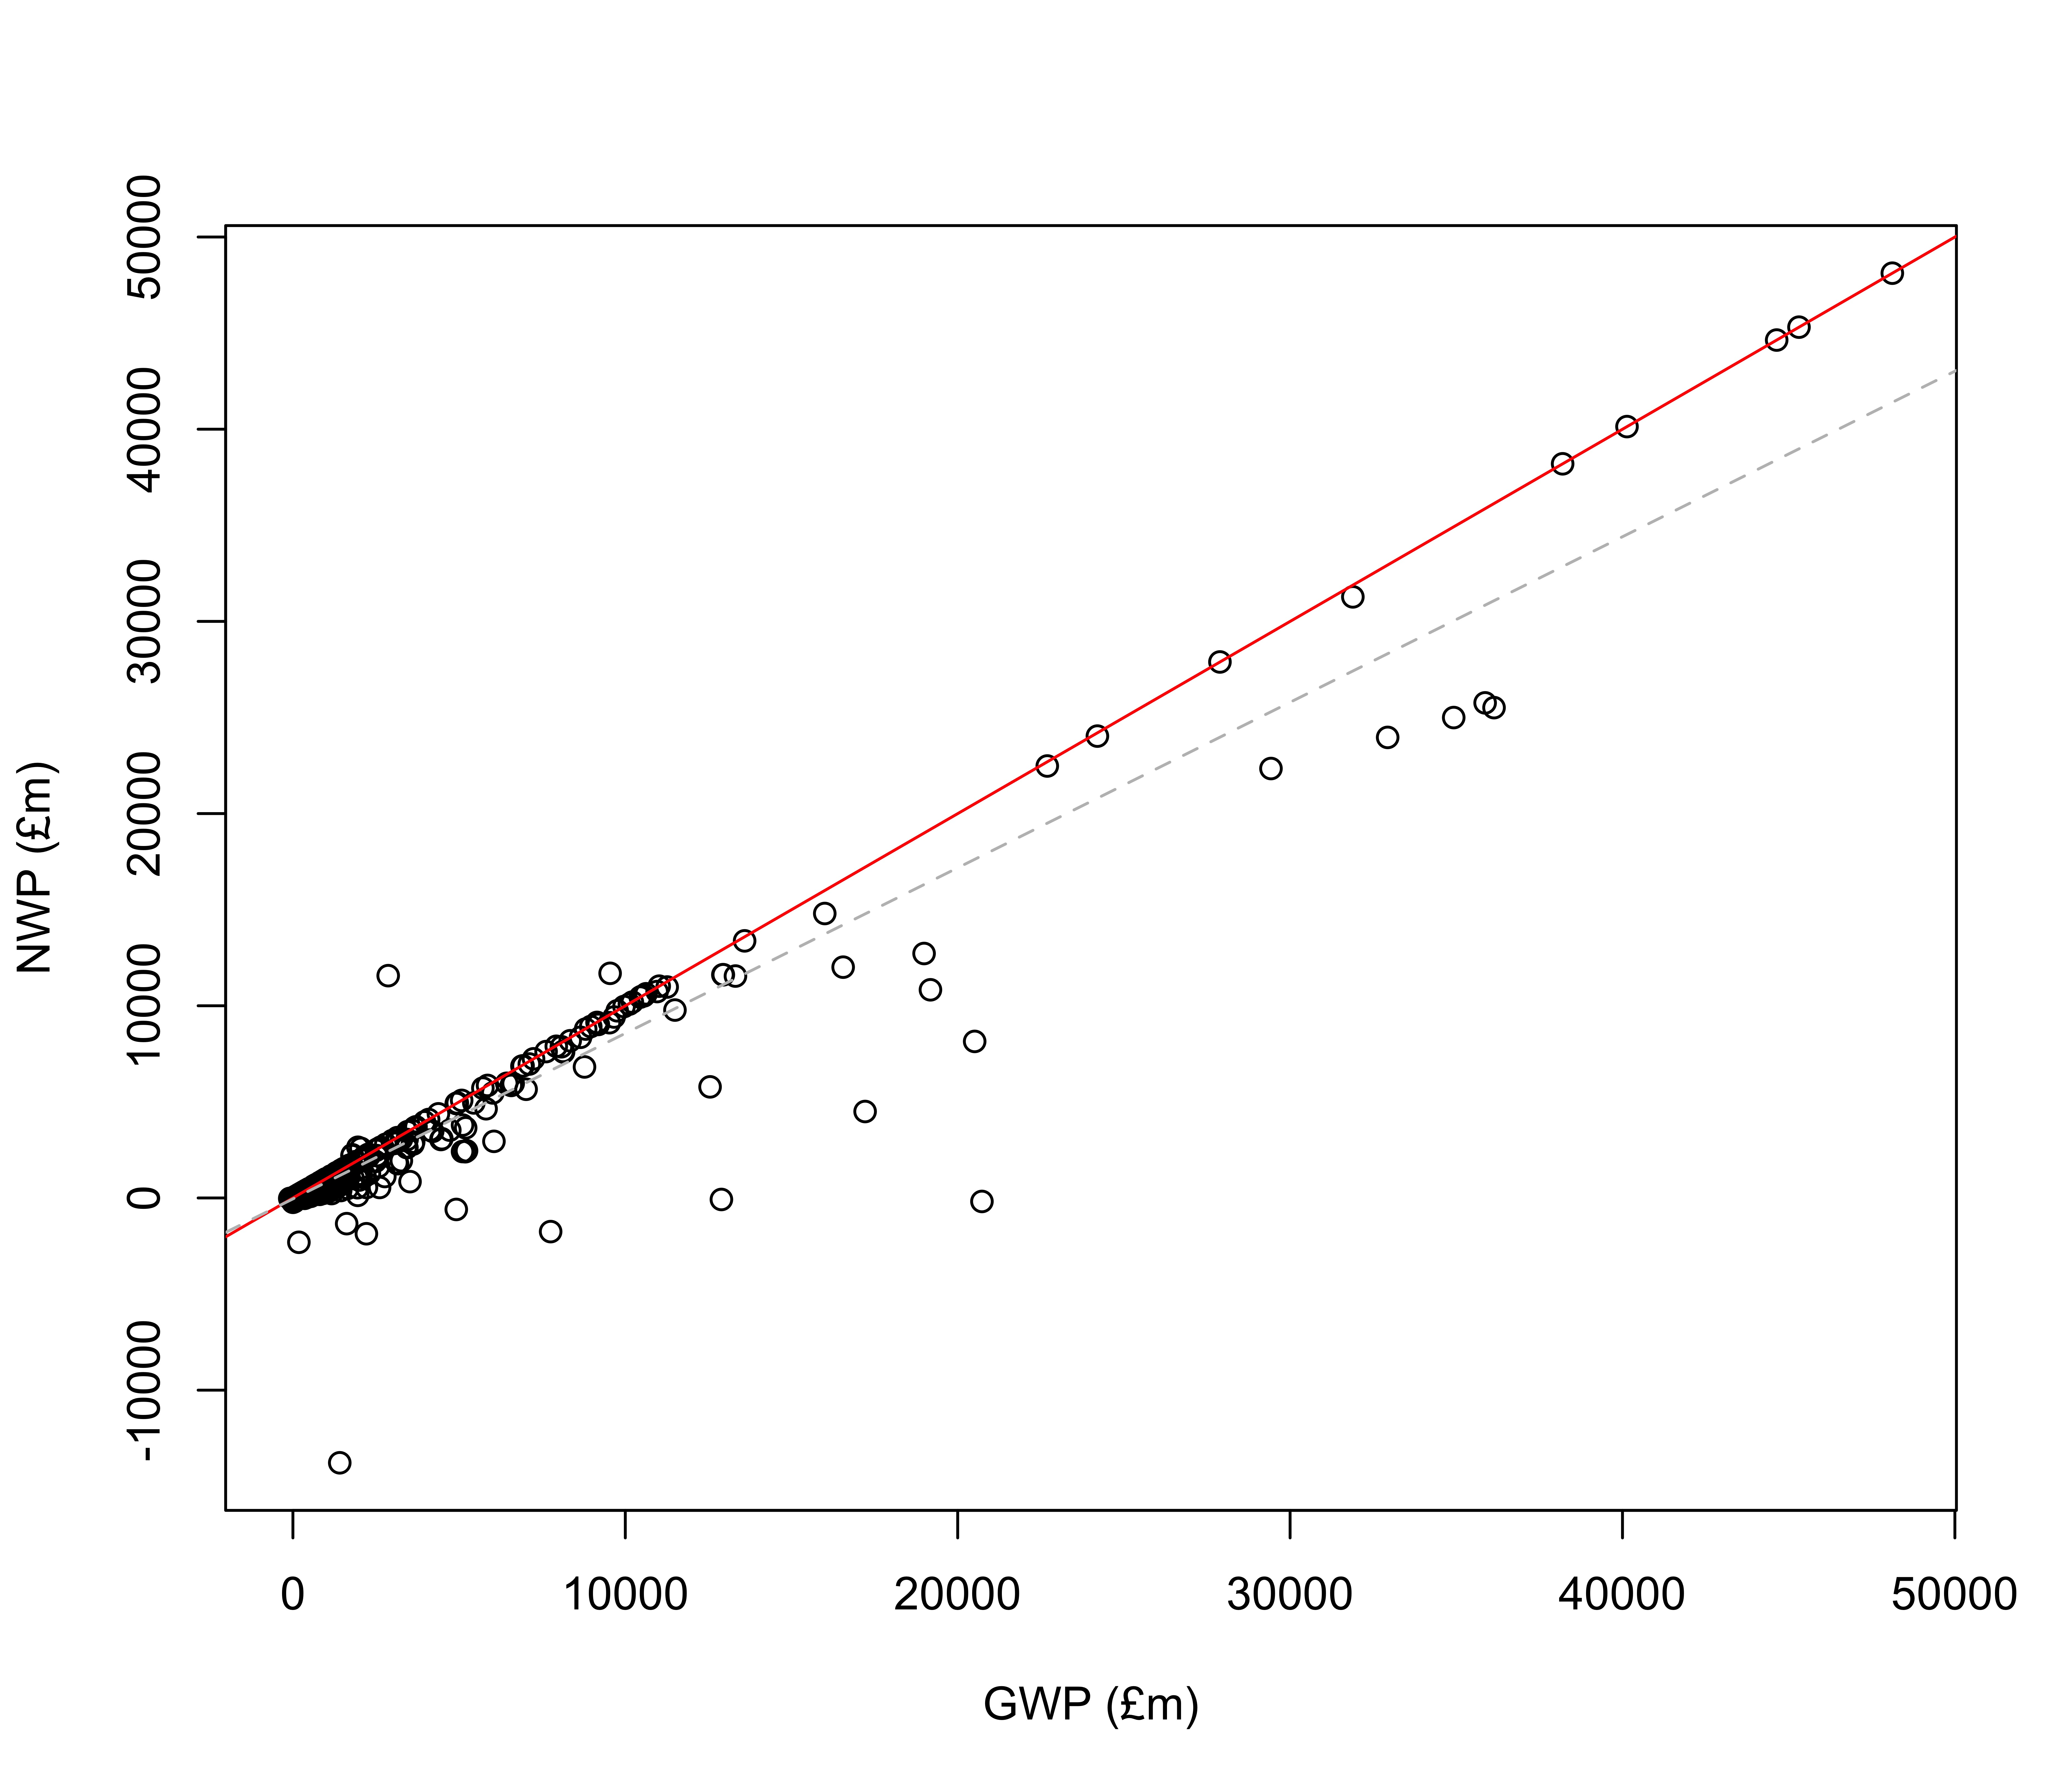
\includegraphics[width=1\linewidth]{../figs/regression_nwp_gwp}

There are 23 firms which are reinsuring 75\% or more, when we look at
mean NWP/GWP for each firm over the four year period. Firms with
negative ratios have been removed.

\begin{longtable}[]{@{}lr@{}}
\toprule
Firm & NWP/GWP \textless{} 0.25\tabularnewline
\midrule
\endhead
Firm 142 & 0.0000000\tabularnewline
Firm 143 & 0.0000000\tabularnewline
Firm 186 & 0.0000000\tabularnewline
Firm 248 & 0.0000000\tabularnewline
Firm 282 & 0.0000000\tabularnewline
Firm 157 & 0.0057308\tabularnewline
Firm 46 & 0.0481001\tabularnewline
Firm 59 & 0.0623781\tabularnewline
Firm 149 & 0.0964830\tabularnewline
Firm 231 & 0.0965117\tabularnewline
Firm 86 & 0.1225895\tabularnewline
Firm 159 & 0.1266646\tabularnewline
Firm 280 & 0.1633861\tabularnewline
Firm 324 & 0.1761774\tabularnewline
Firm 45 & 0.2208831\tabularnewline
Firm 292 & 0.2317231\tabularnewline
Firm 286 & 0.2433416\tabularnewline
Firm 61 & 0.2481371\tabularnewline
\bottomrule
\end{longtable}

\hypertarget{scr-coverage-ratio}{%
\subsubsection{SCR Coverage Ratio}\label{scr-coverage-ratio}}

272 out of the 325 firms have across the four year period an average of
more than 100\%, and so are therefore meeting prudential capital
requirements. Some have values much higher than 100\%. These are
displayed below.

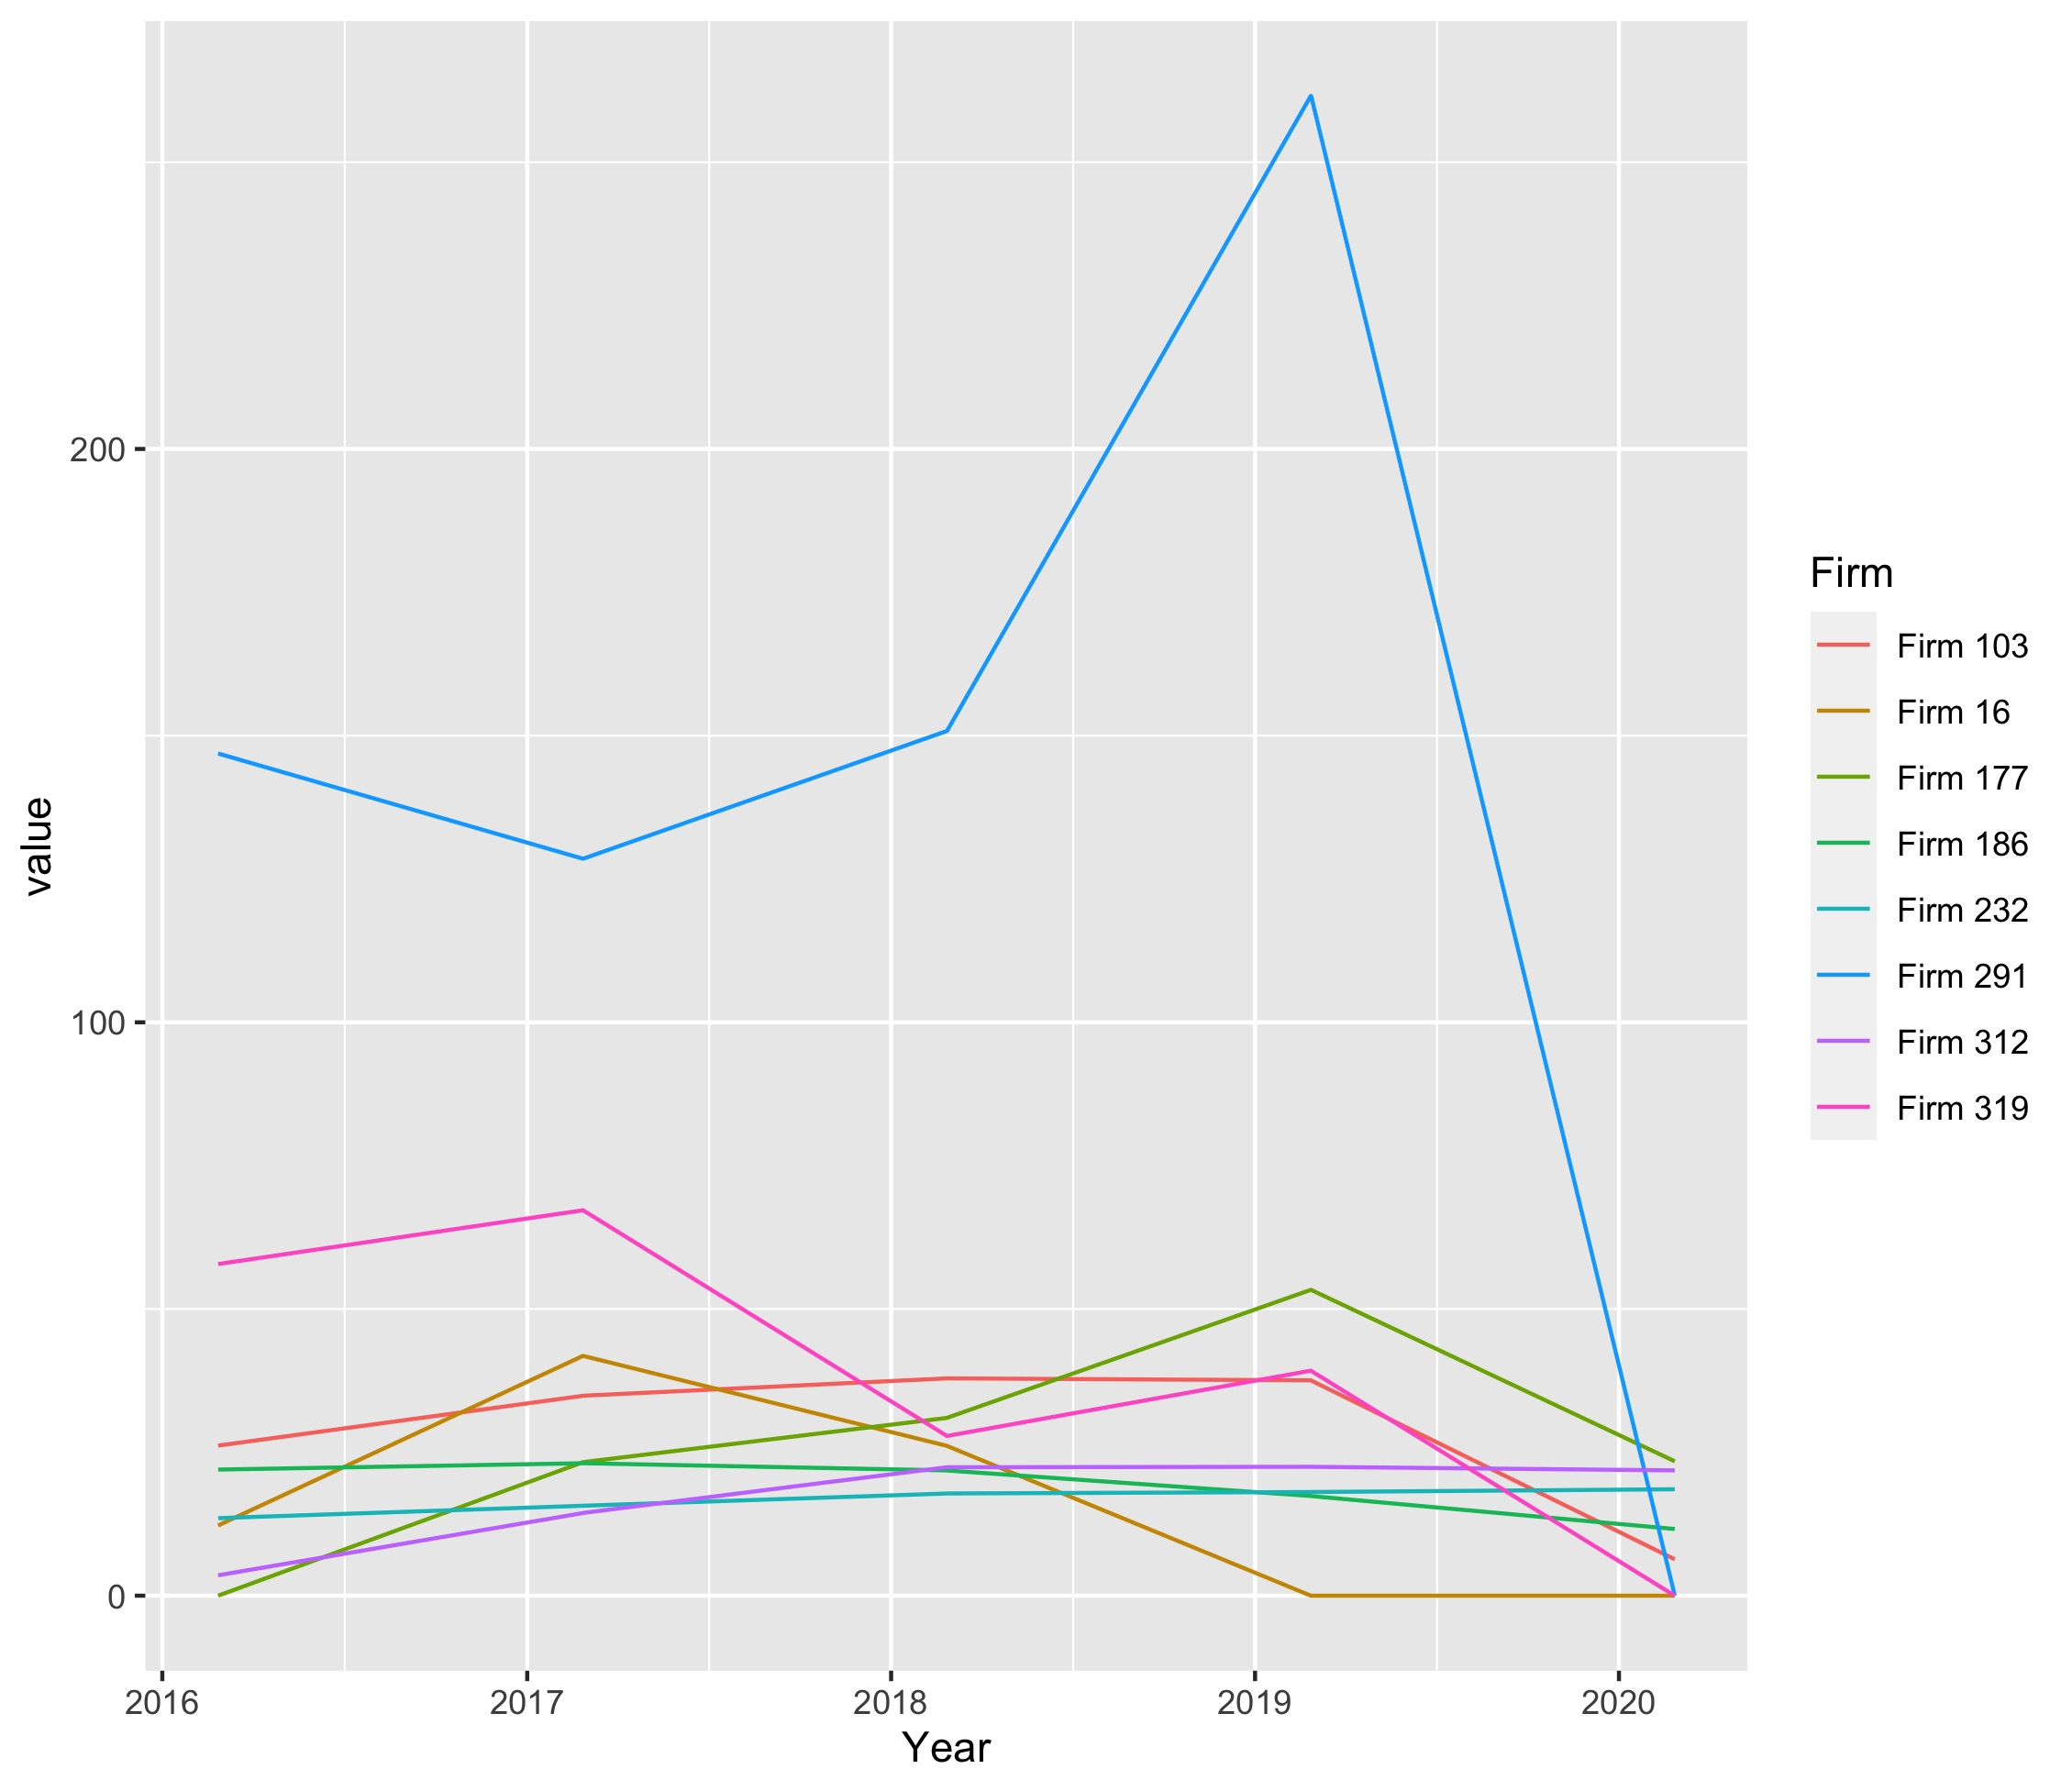
\includegraphics[width=1\linewidth]{../figs/high_scr_plot}

This figure is presented on filtered data where the average SCR ratio
over the four year period was higher than 1500\% but lower than
1,000,000\%. In particular we see high variability in firm 291. We can
also present the firms with the very highest SCR ratio. This table below
shows firms, by year, where the SCR ratio was higher than 1,000,000\%.
These firms might be considered outliers in this data set.

\begin{longtable}[]{@{}lrl@{}}
\toprule
Firm & SCR ratio & Year\tabularnewline
\midrule
\endhead
Firm 216 & 963584000.0 & 2017-02-26\tabularnewline
Firm 1 & 481792000.0 & 2017-02-26\tabularnewline
Firm 131 & 481792000.0 & 2017-02-26\tabularnewline
Firm 320 & 4181573.0 & 2016-02-26\tabularnewline
Firm 66 & 3856018.2 & 2018-02-26\tabularnewline
Firm 127 & 194753.8 & 2018-02-26\tabularnewline
Firm 127 & 182412.2 & 2017-02-26\tabularnewline
Firm 127 & 171974.7 & 2019-02-26\tabularnewline
Firm 127 & 166394.6 & 2020-02-26\tabularnewline
\bottomrule
\end{longtable}

\hypertarget{gross-claims-incurred-gci}{%
\subsubsection{Gross Claims Incurred
(GCI)}\label{gross-claims-incurred-gci}}

128 firms have GCI less than £1 million on average across the four
years. These firms, representing over a third of the data set are
excluded subsequently. The largest firms display a variety of temporal
dynamics. Some firms remain relatively stable (E.g. Firm 22, 234), while
others drop precipitously over time (e.g.~Firm 216), and yet others are
more variable (e.g.~Firm 17 which drops and then increases).

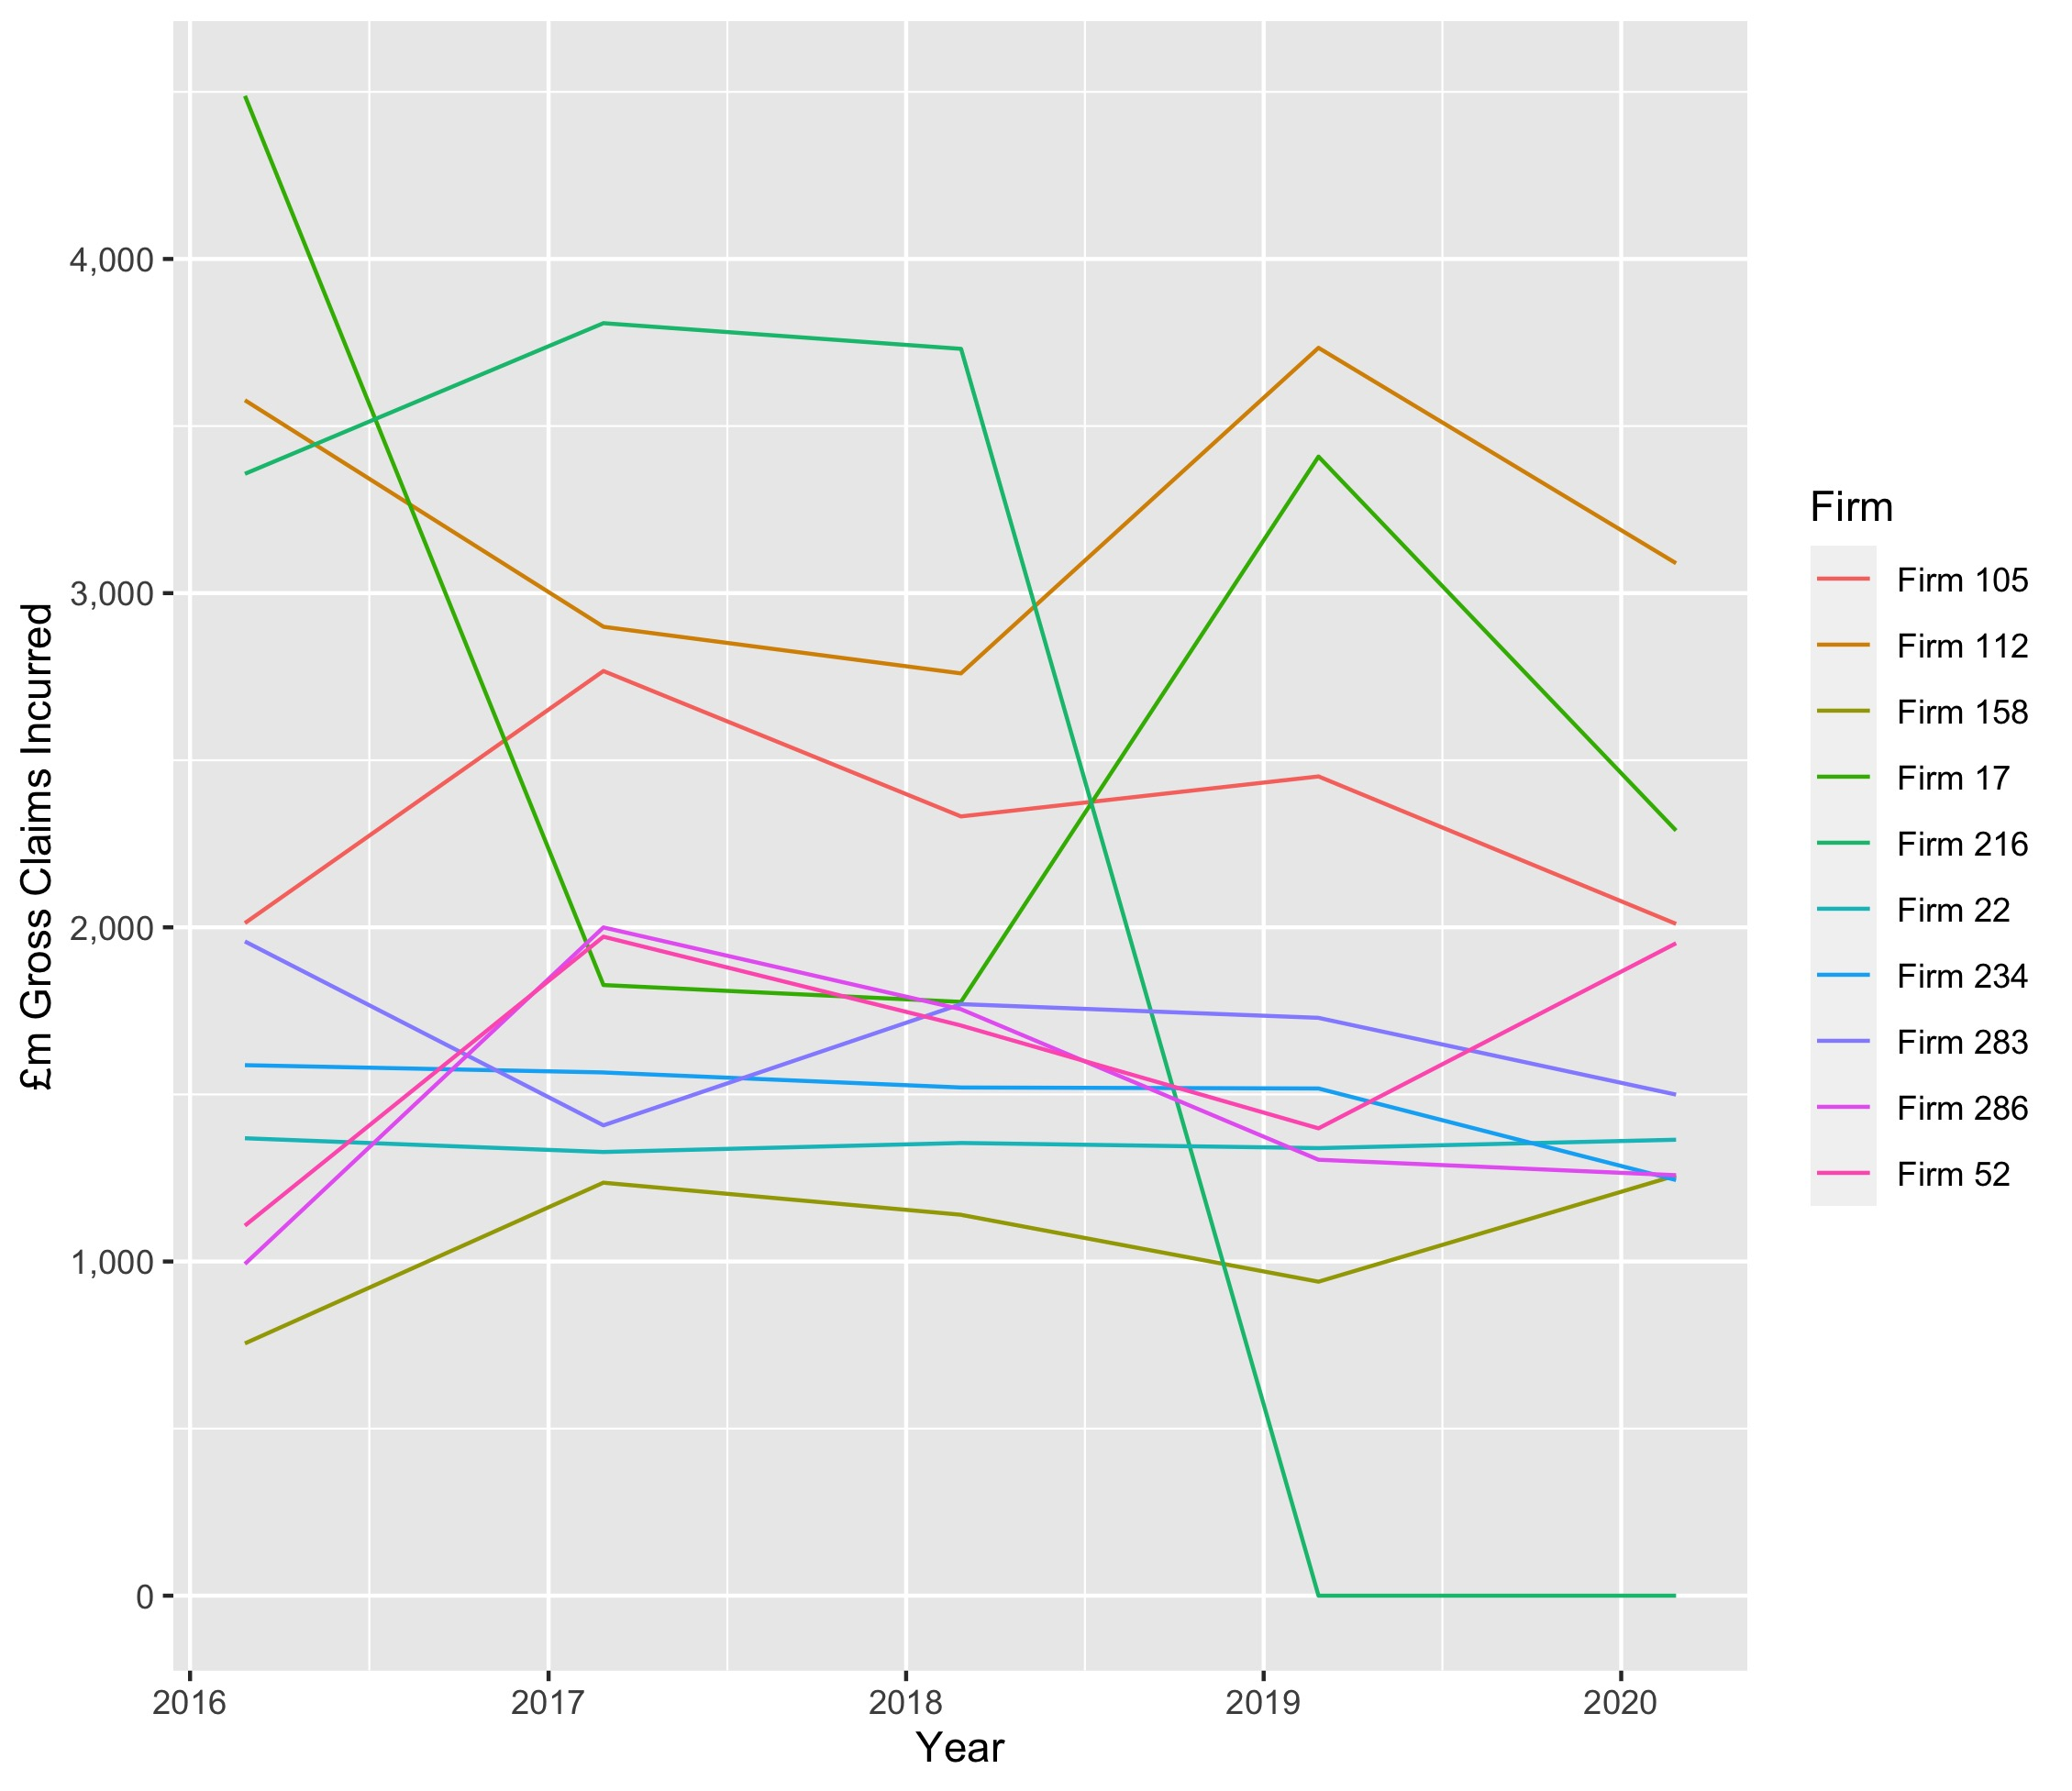
\includegraphics[width=1\linewidth]{../figs/gross_claims_incurred_plot}

If we again look at variance through time as we did for GWP, four firms
show high variability but are not shown in the plot above. These are
Firms 200, 25, 304, and 49. Each of these firms increase in GCI, then
drop.

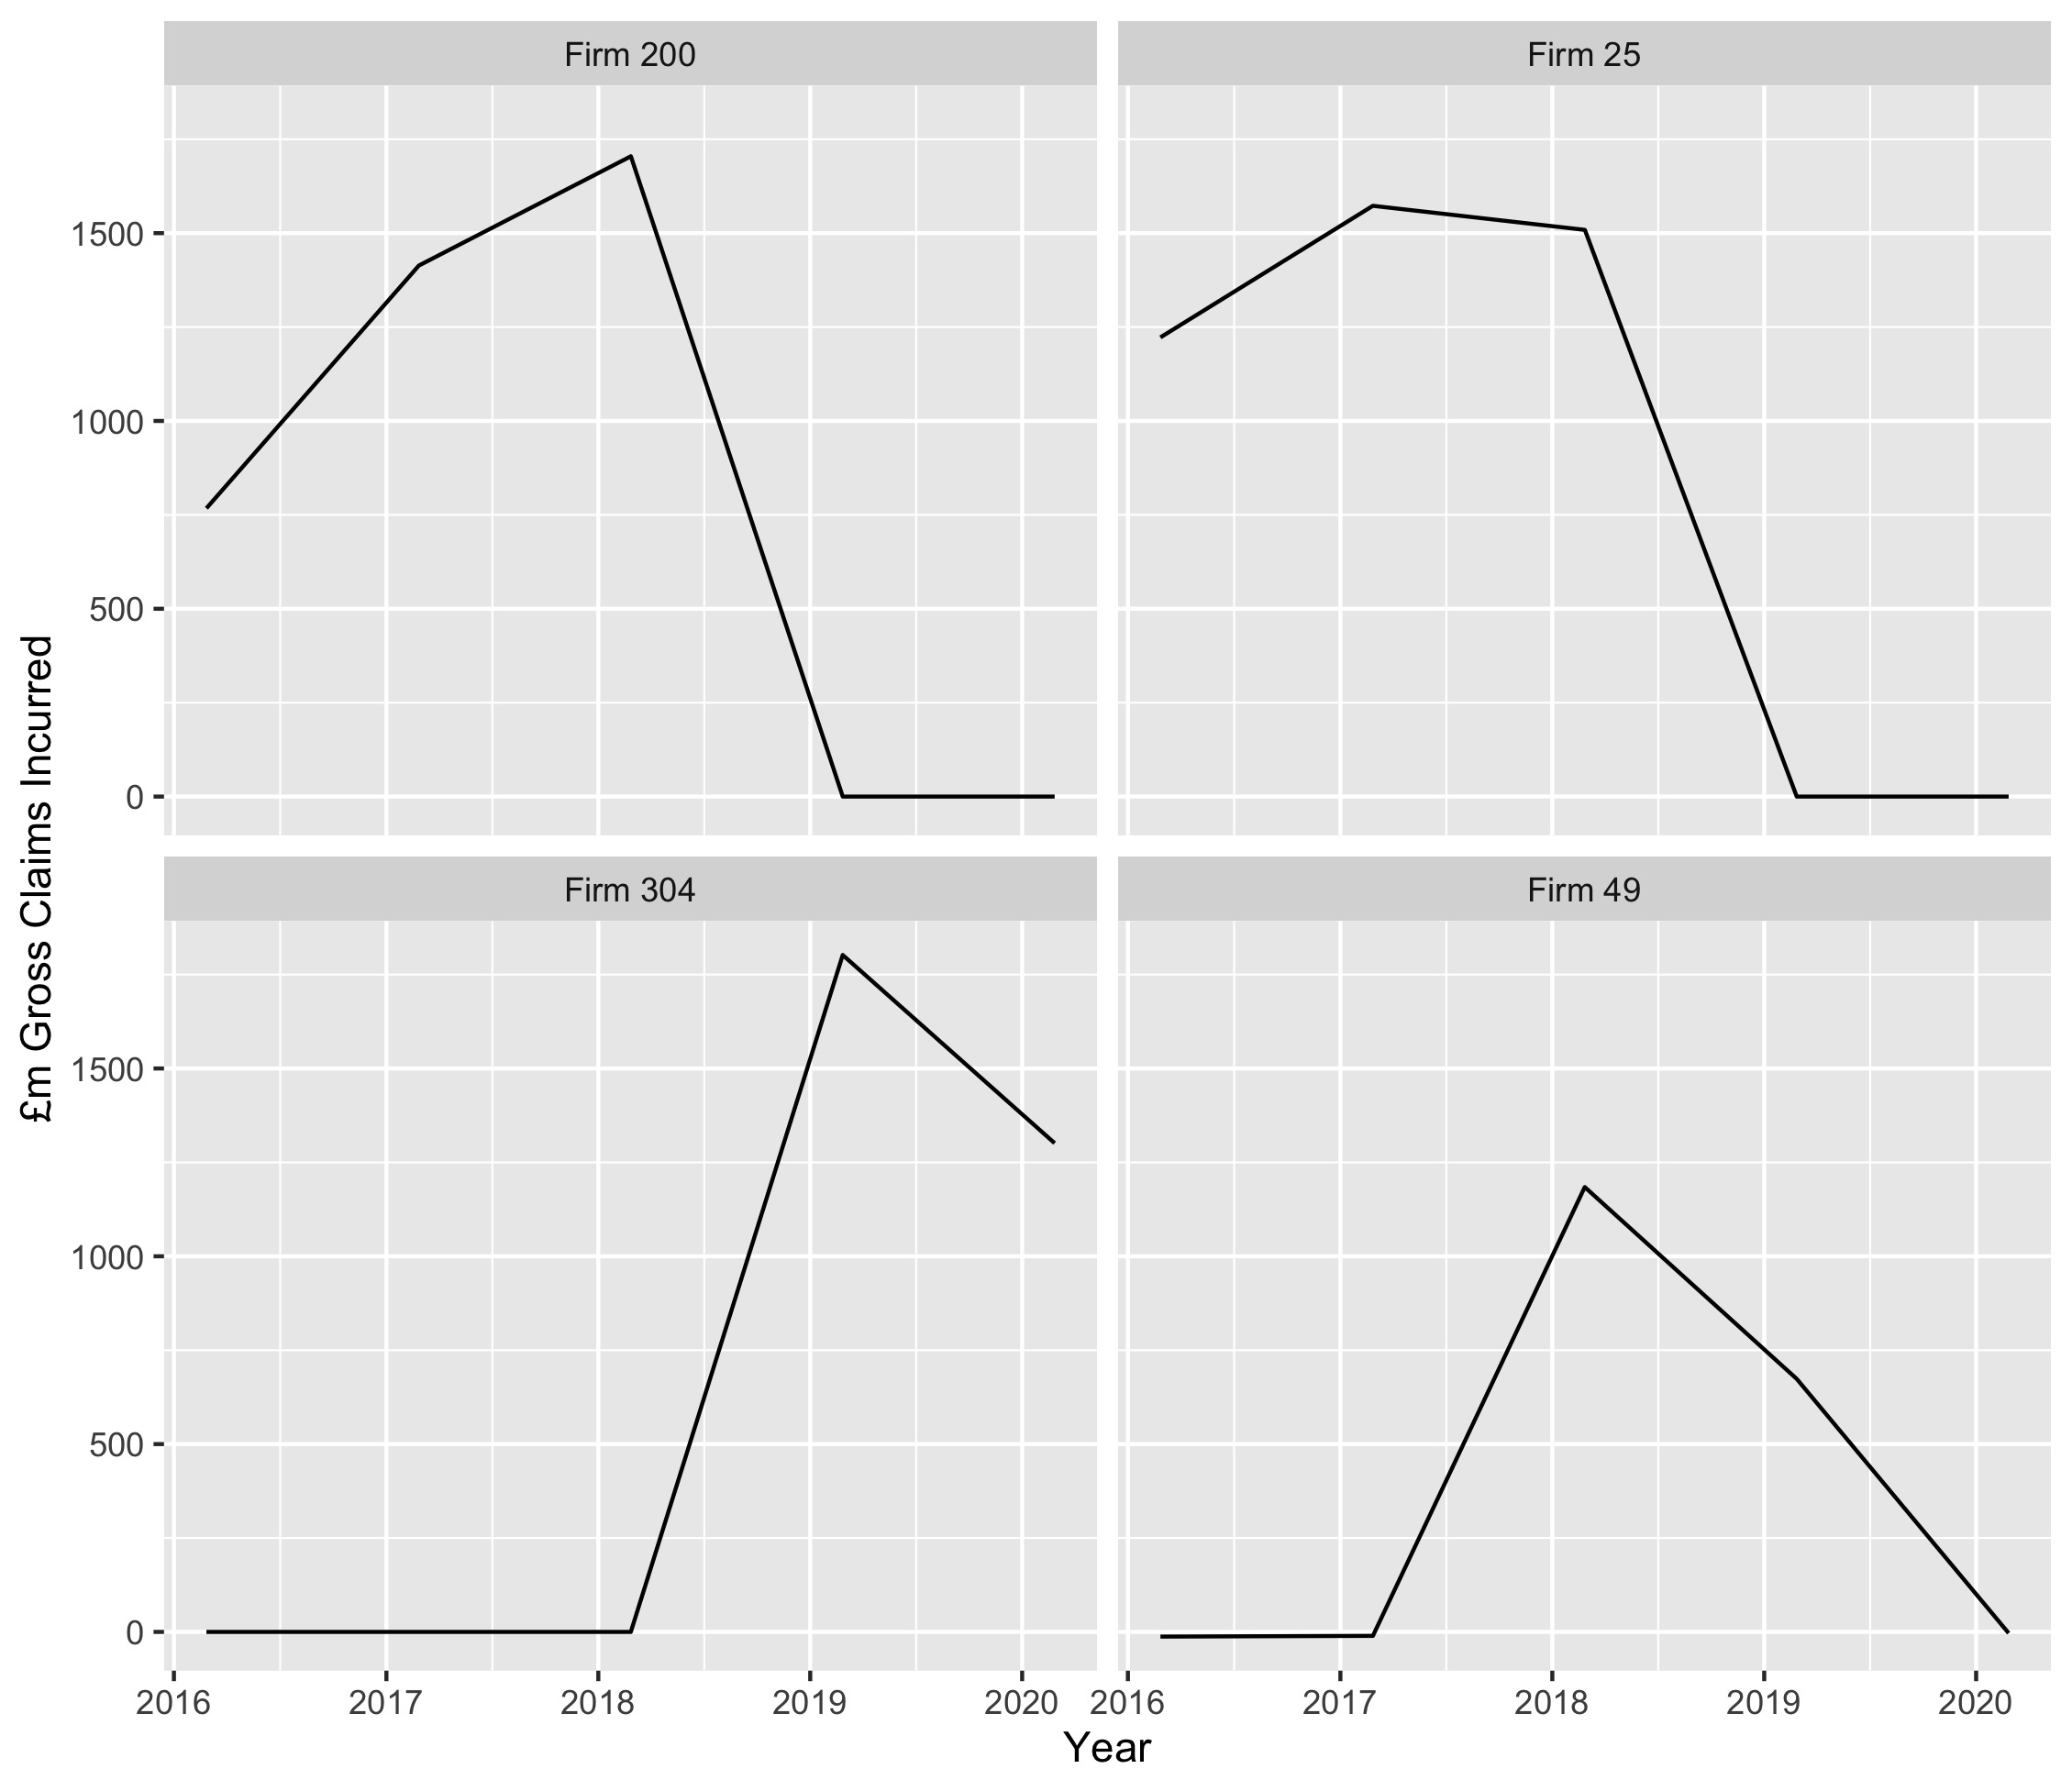
\includegraphics[width=1\linewidth]{../figs/variable_gci_plot}

\hypertarget{net-combined-ratio-nci}{%
\subsubsection{Net combined ratio (NCI)}\label{net-combined-ratio-nci}}

A simple histogram of NCI across all firms and years can be informative.
There is an apparent normal distribution with a mean of 1, indicating
that the average NCI across many firms and years have an equilibrium of
losses and earned premiums. The spike at zero may be because of no
earned premiums for a firm in that particular year (this seems to be
frequent). Values that lie beyond this plot are considered outliers.

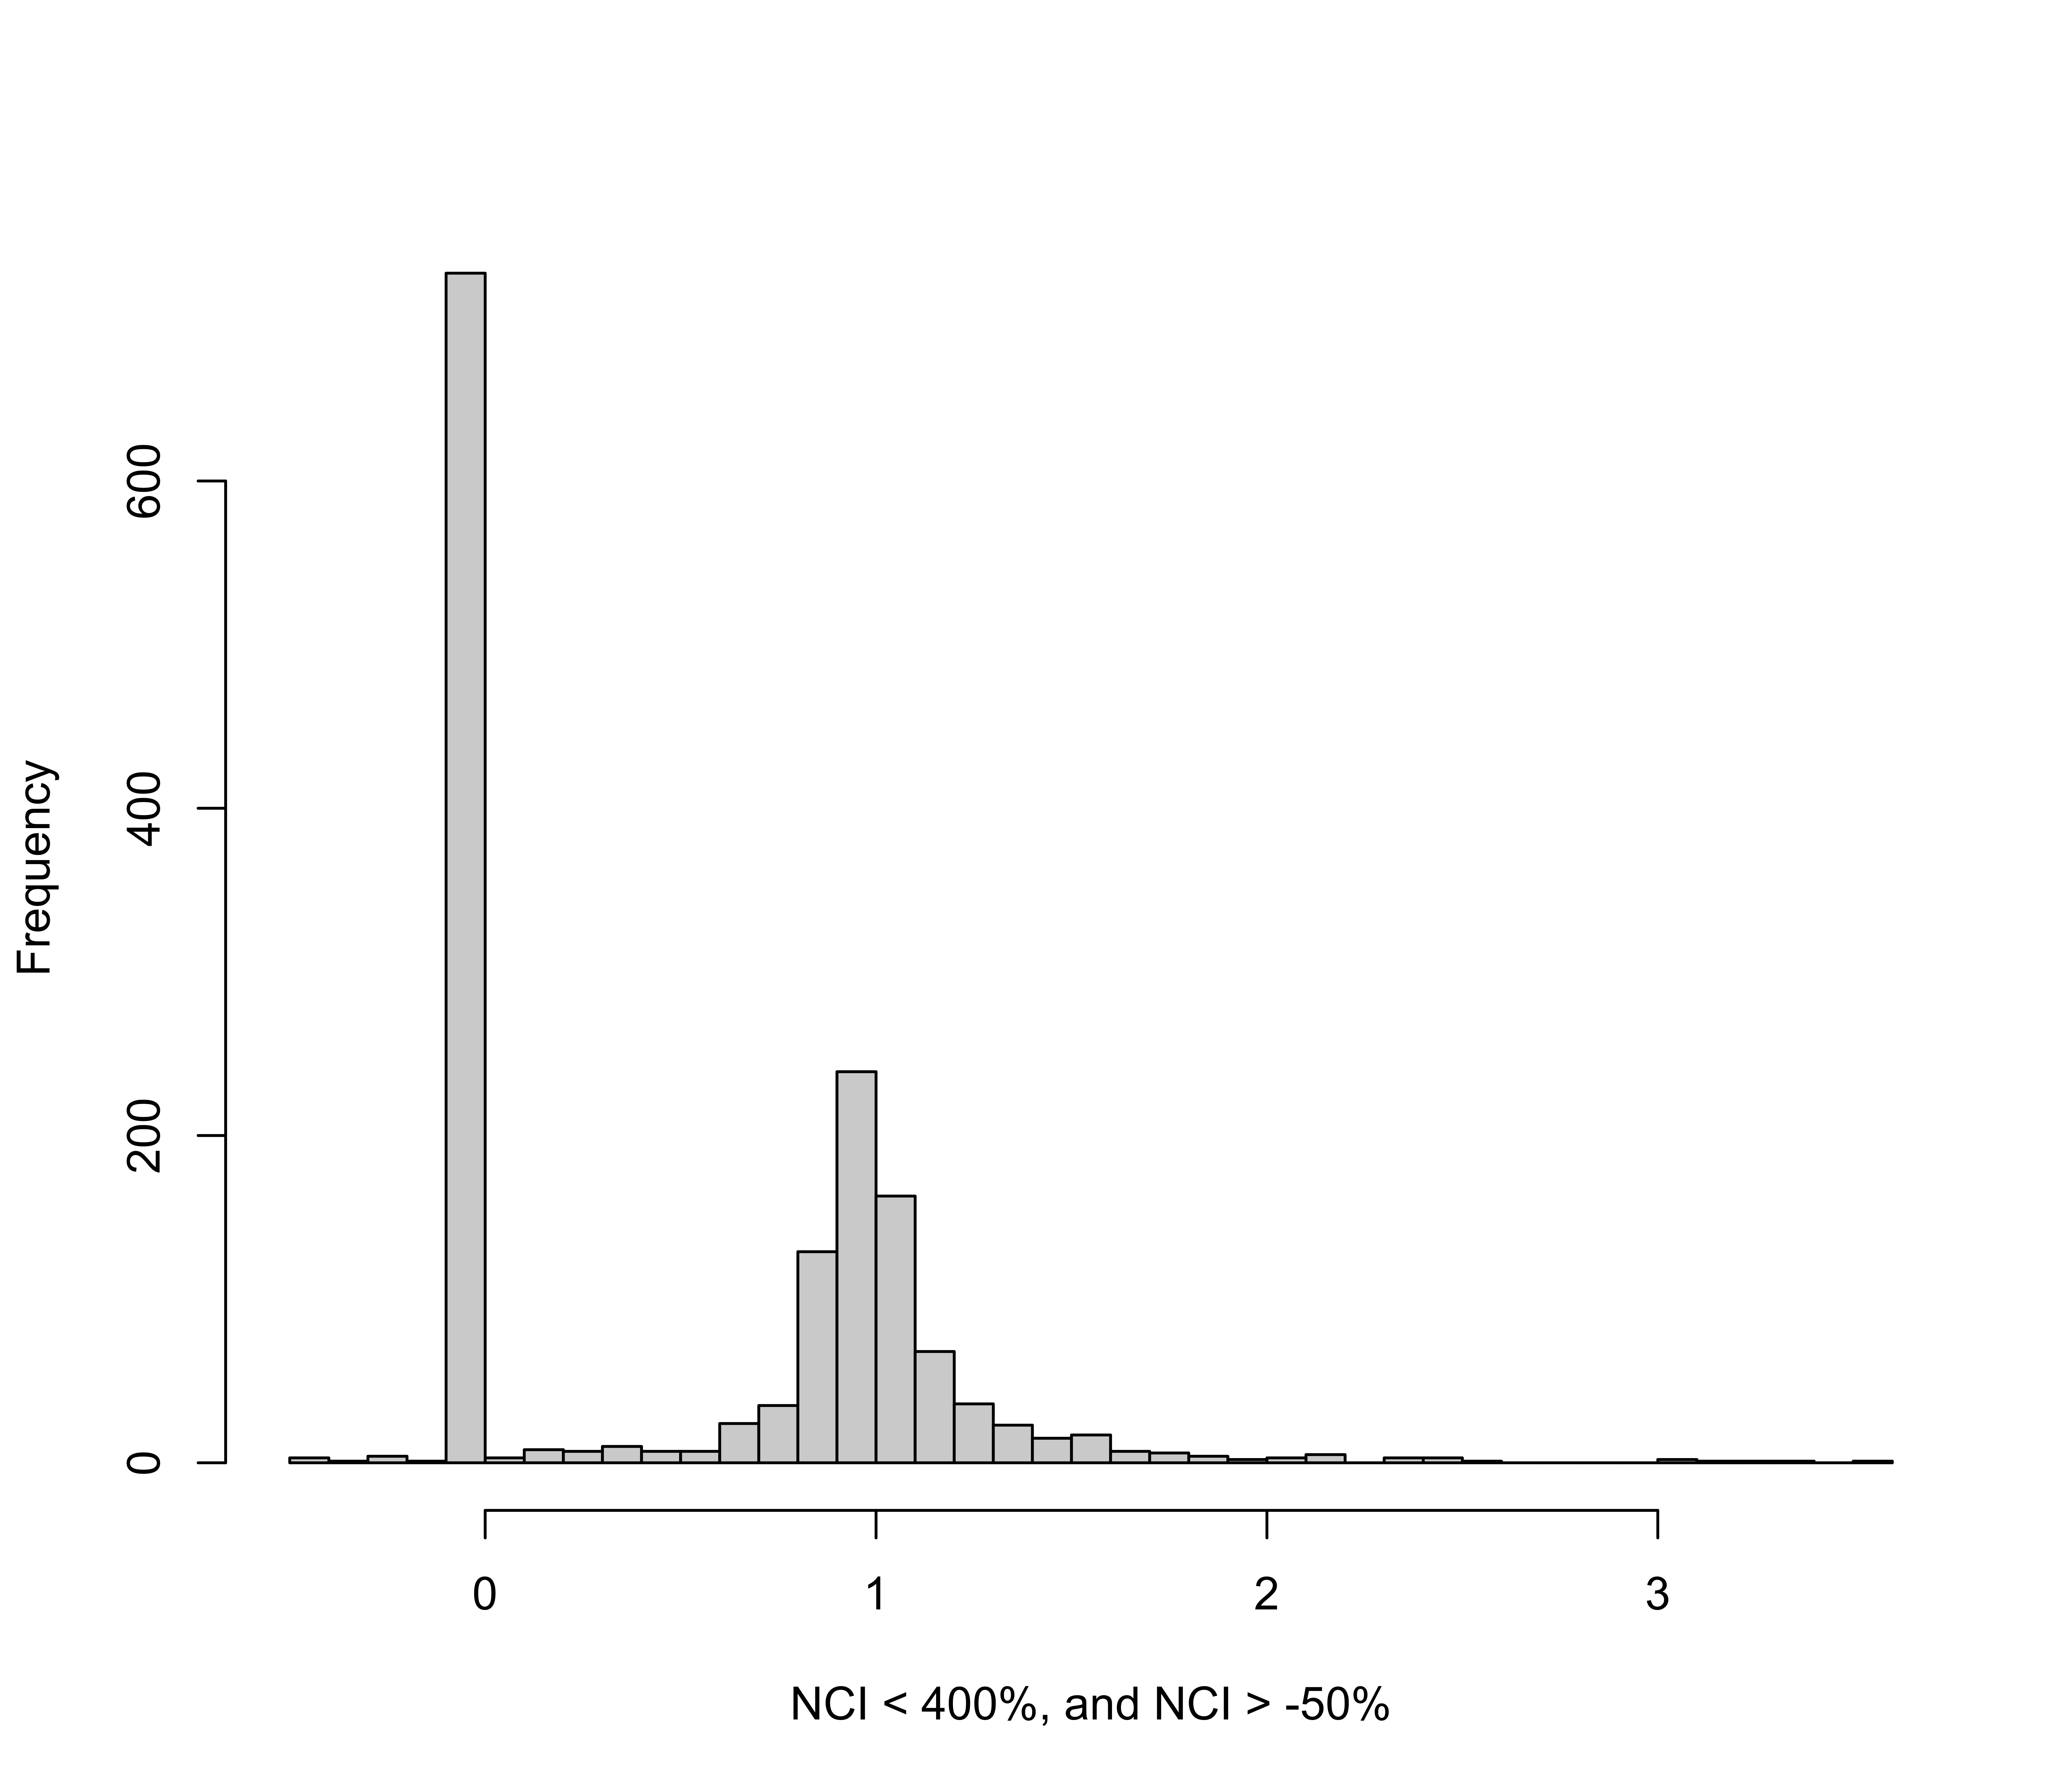
\includegraphics[width=1\linewidth]{../figs/hist_nci}

If we again visualise over time, but filter for firms which have more
than 0\% NCI and less than 80\% NCI across all years, we find very few
firms fitting these criteria. In particular, Firm 247 appears to have a
very low NCI.

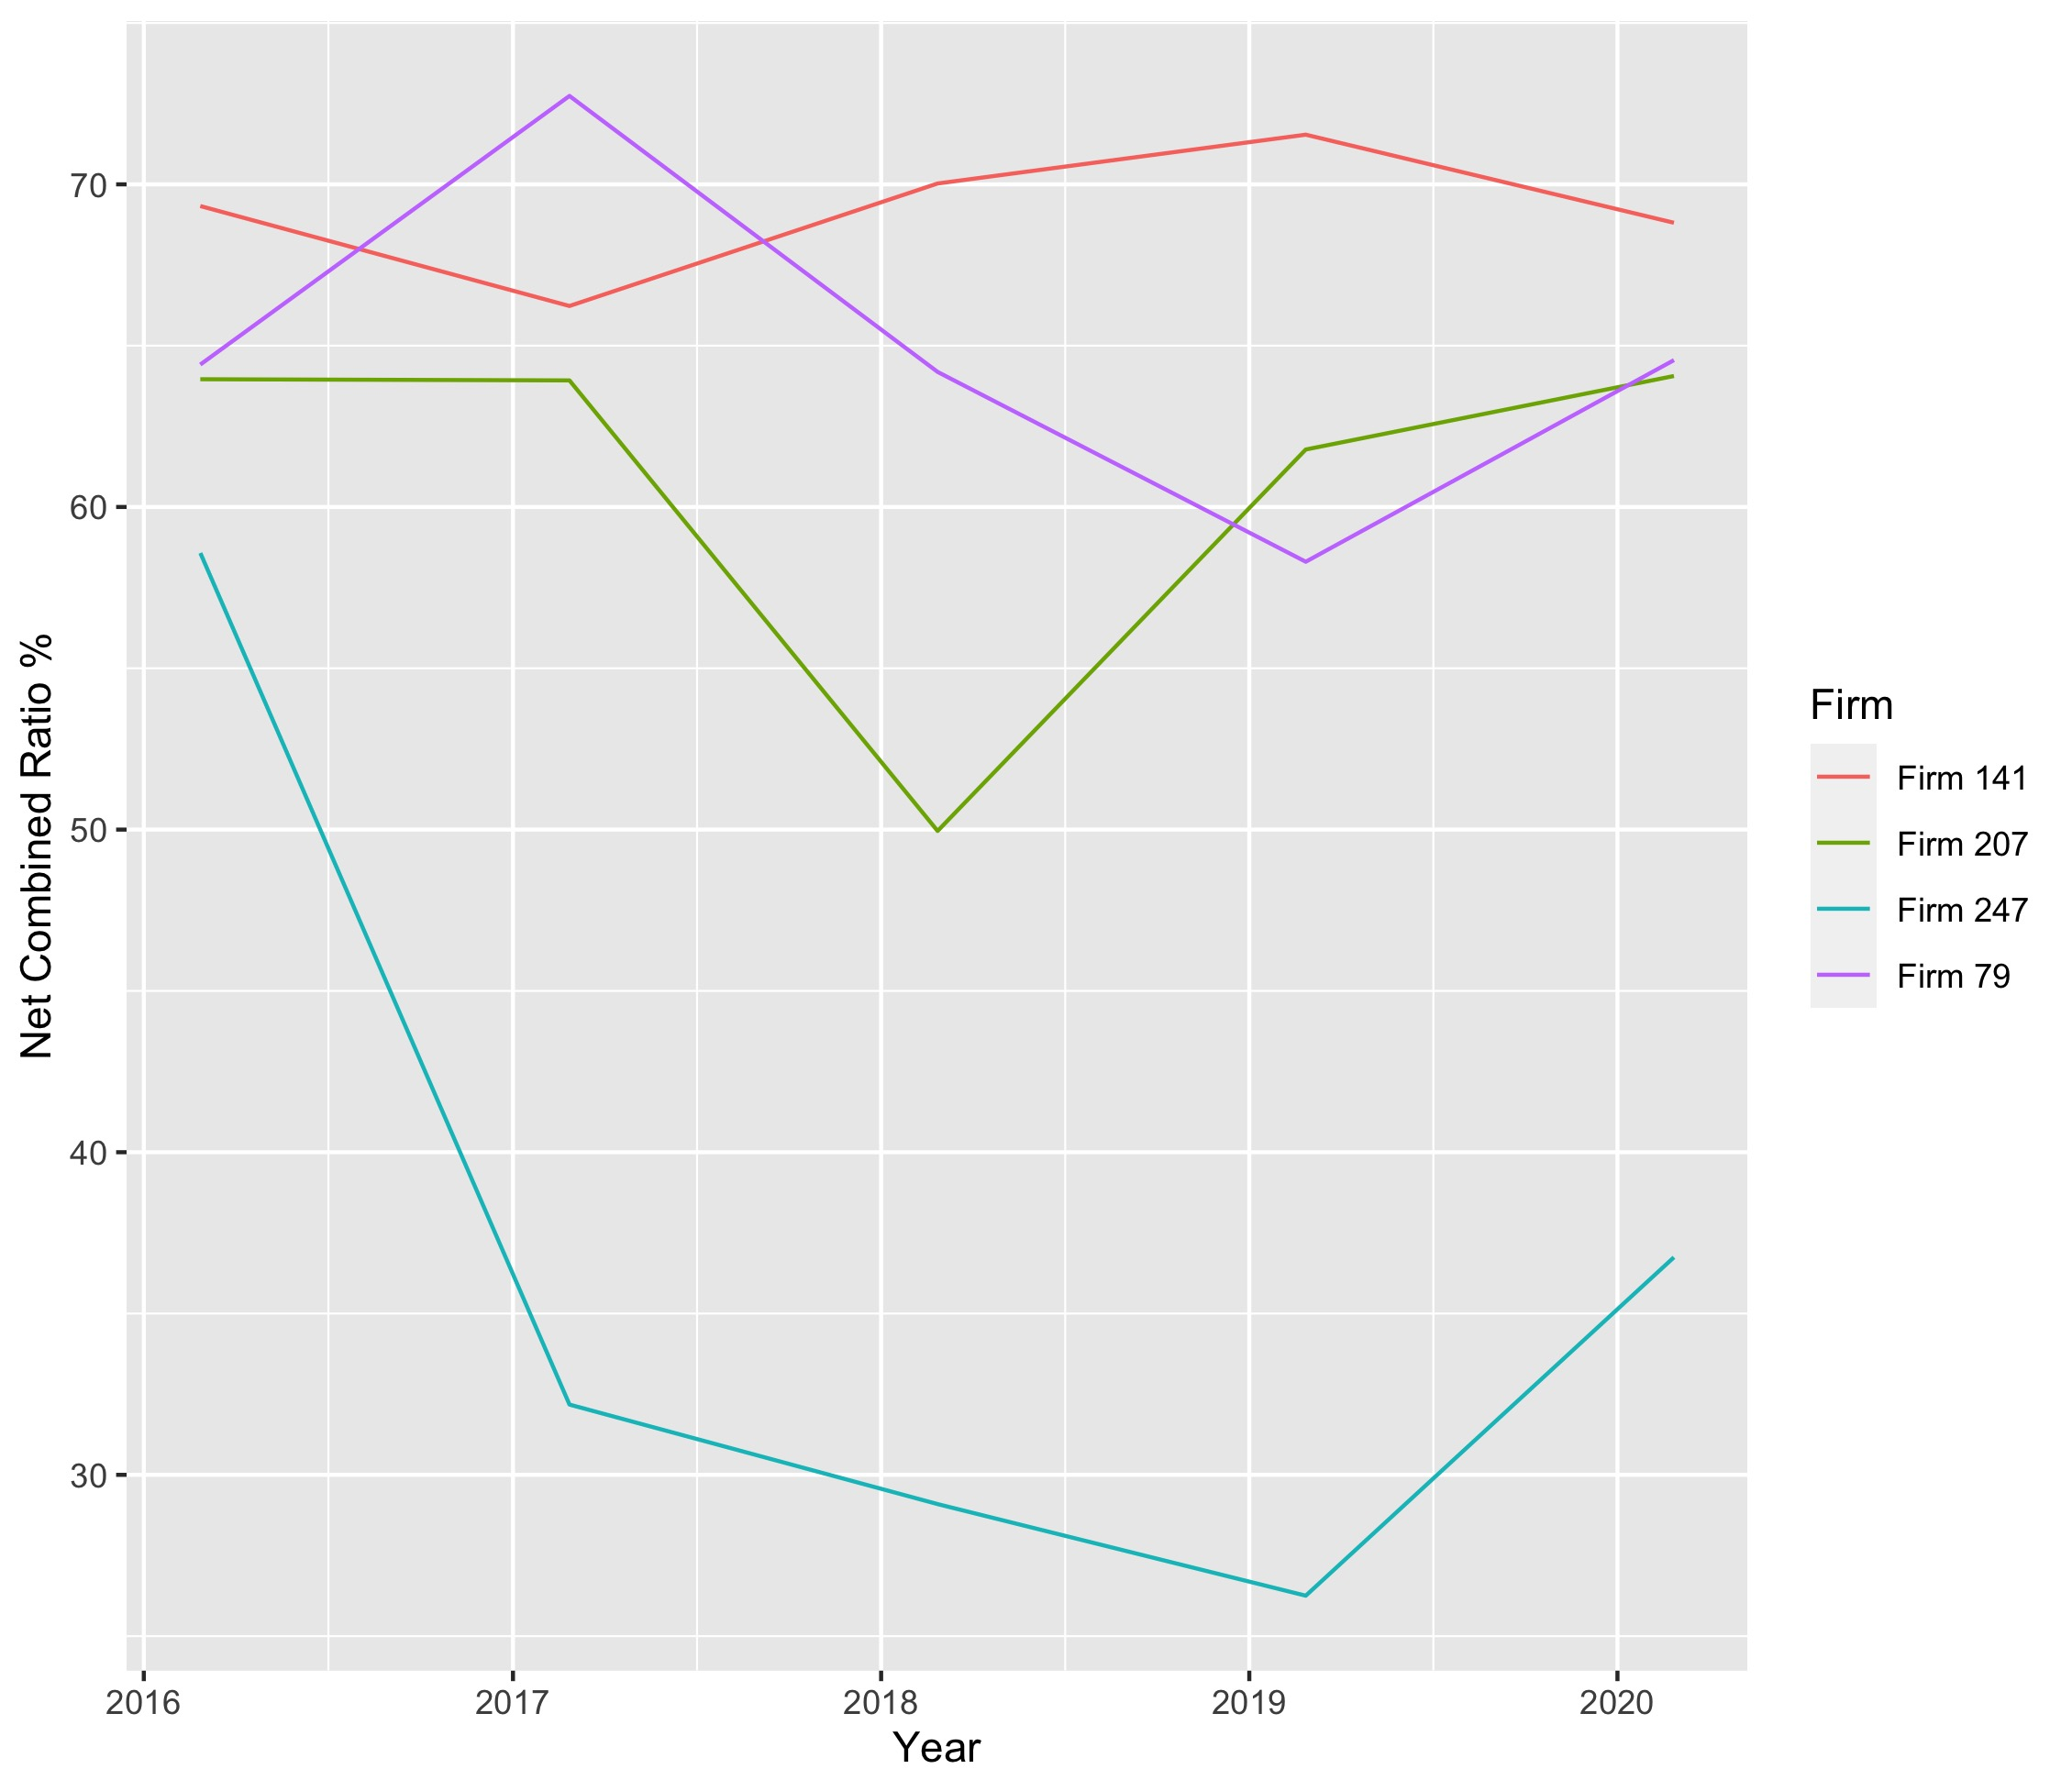
\includegraphics[width=1\linewidth]{../figs/net_combined_ratio_minus_outliers_plot}

\hypertarget{summary}{%
\subsubsection{Summary}\label{summary}}

The largest firms which average over a billion £GWP each year should be
investigated, which are highlighted in the GWP section. Firm 26 in
particular shows a large drop in GWP. Although GWP and NWP are
correlated, firms which fall below the line of best fit are reinsuring
relatively more than other firms. These firms can be easily isolated. In
addition, I provide a table to look at those firms which on average over
time are reinsuring over 75\%. Some firms appear to be reinsuring at
100\%.

The SCR coverage ratio represents an interesting variable. Excluding
outliers, firm 291 warrants further investigation. If we include
outliers however, there are some extremely high SCR coverage ratios
present in this data set. Firm 216 spikes in 2017 at over 96 billion
percent, which could be an error in the data. Firm 127 has consistently
very high SCR coverage ratio.

For GCI, four firms in particular display interesting temporal dynamics
(Firms 200, 25, 304, 49), with peaks and declines in this variable.
Lastly, NCI shows a bimodal distribution, and after drilling down
presents another four firms which would be worth investigating further.

\hypertarget{annex-machine-learning}{%
\subsection{Annex: Machine Learning}\label{annex-machine-learning}}

To gain a more holistic overview of the data set, a useful and commonly
used Machine Learning (ML) technique is the Principal Component Analysis
(PCA). A PCA tries to explain the variability in a lower number of
dimensions than the data set, so it can be visualised. For example, we
can combine both data sheets provided, and average across years (move
the effect of year to a single data point) to simplify the data. We can
then run a PCA across all these 18 variables.

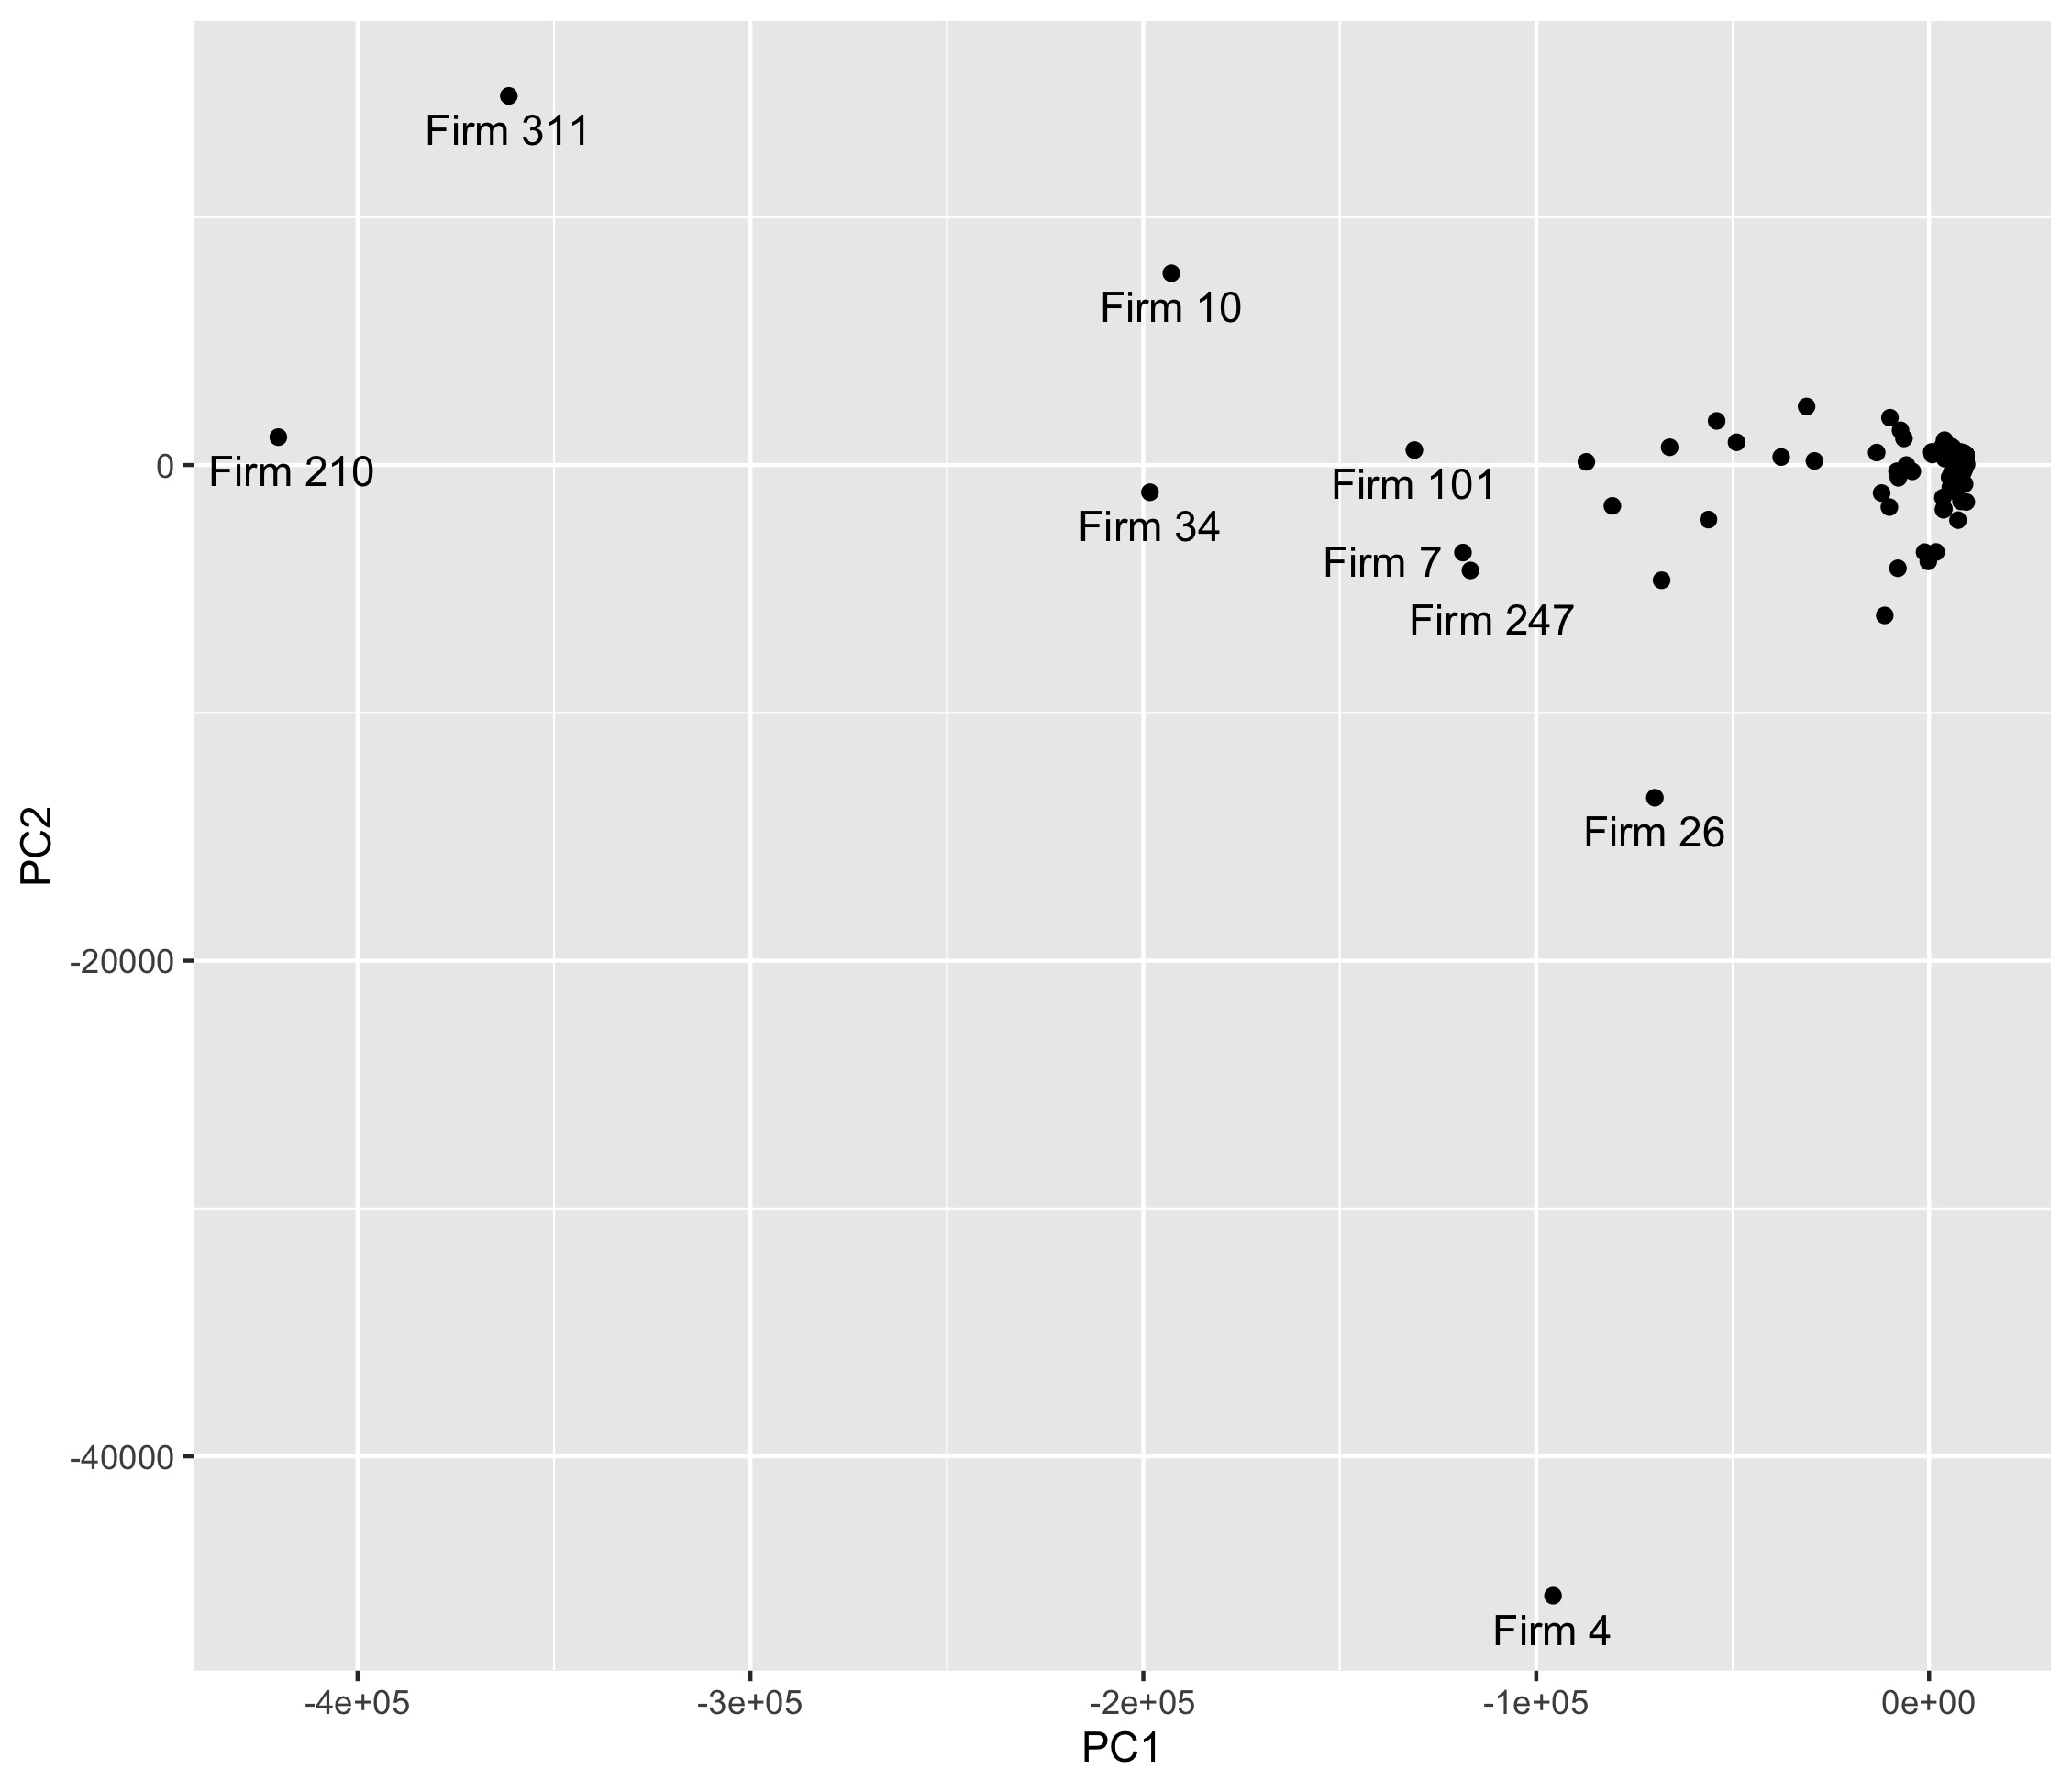
\includegraphics[width=1\linewidth]{../figs/pca_plot}

I have highlighted some firms which appear to deviate highly from the
main cluster of points in the top right. Some of these firms (e.g.~210)
were already known to us from the above analysis. Others, e.g.~Firm 7,
have not yet been highlighted and so may be worth investigating for
other reasons.

Based on the available series of annual firm data, rules and limits can
be derived by periodic inspection. These rules can be applied to
existing Supervisory tools to forecast and predict potential SCR risks
and other regulatory conditions.

The production of these rules and limits could be validated through a
set of R scripts to produce results and outputs to save supervisory time
and enhance processes.

\end{document}
